\documentclass[10pt,a4paper]{article}

\newcommand{\COLORSDIR}{/Users/hoolywear/Desktop/UNIMORE/II ANNO/II SEMESTRE/colors}

\usepackage[italian]{babel}
\usepackage[usenames,dvipsnames,table]{xcolor}
\usepackage[utf8]{inputenc}
\usepackage[T1]{fontenc}
\usepackage{soul}
\usepackage[a4paper, portrait, margin=2.5cm]{geometry}
\usepackage{array}
\usepackage{tabularx}
\usepackage{multicol}
\usepackage{amsmath}
\usepackage{amsfonts}
\usepackage{amssymb}
\usepackage{algorithmicx}
\usepackage[noend]{algpseudocode}
\usepackage{wrapfig}
\usepackage{graphicx}
\usepackage{hyperref}
\hypersetup{
    colorlinks=true,
    linkcolor=black,
    filecolor=magenta,      
    urlcolor=cyan,
    pdftitle={Overleaf Example},
    pdfpagemode=FullScreen,
    }
\urlstyle{same}
\usepackage{caption}
\usepackage{capt-of}
\captionsetup[figure]{name=Fig.}
\renewcommand{\thefigure}{\arabic{section}.\arabic{figure}}
\graphicspath{ {./images/} }

\input{\COLORSDIR/colors_4}

\usepackage{listings}

\definecolor{codeblue}{HTML}{1e66f5}
\definecolor{codepurple}{HTML}{8839ef}
\definecolor{codered}{HTML}{d20f39}
\definecolor{darkbluenord}{HTML}{232731}
\definecolor{lightbluenord}{HTML}{b1bfe3}

\lstdefinestyle{code}{
    backgroundcolor=\color{gray!10},   
    basicstyle=\ttfamily,
    commentstyle=\color{codeblue},
    keywordstyle=\color{codered},
    breakatwhitespace=false,         
    breaklines=true,                 
    captionpos=b,                    
    keepspaces=true,                 
    showspaces=false,                
    showstringspaces=false,
    showtabs=false,                  
    tabsize=2,
    mathescape=true %dollar signs act as inline math delimiters
}

\lstdefinestyle{python}{
    style=code,
    language=python,
    commentstyle=\color{codeblue},
    keywordstyle=\color{codepurple},
    stringstyle=\color{codered}
}

\lstset{style=code,language=C++}

\usepackage[framemethod=TikZ]{mdframed}

\mdfsetup{%
  roundcorner=8pt}

% styles
\def\Clinewidth{.8pt}
\mdfdefinestyle{titlerule}{%
  frametitlerule=true,%
  frametitlerulewidth=\Clinewidth,%
  subtitleaboveline=true,subtitlebelowline=true,%
  subtitleabovelinewidth=\Clinewidth,subtitlebelowlinewidth=\Clinewidth,%
linewidth=1pt}

\mdfdefinestyle{emphasize}{%
  style=titlerule,%
  frametitle=,%
  linecolor=gray!50,linewidth=1pt,backgroundcolor=gray!10}

% algorithmic environment
\surroundwithmdframed[backgroundcolor=gray!10,hidealllines=true,%
frametitle={}]{algorithmic}

% quote environment
\surroundwithmdframed[style=emphasize]{quote}

% example environment
\newmdenv[frametitle=Esempio,style=titlerule]{example}

% emphasize environment
\newmdenv[style=emphasize,%
          linecolor=emp!70!red,backgroundcolor=emp]{emphasize}

% blue emphasize environment
\newmdenv[style=emphasize,%
          linecolor=obs!70,backgroundcolor=obs!20]{emphasize-blue}

%% NOT USED IN III ANNO
%% % definition environment
%% \newmdenv[frametitle=Definizione,style=titlerule,%
%%           linecolor=def]{definition}
%% 
%% % theorem environment
%% \newmdenv[frametitle=Teorema,style=titlerule,%
%%           linecolor=the]{theorem}
%% % observation environment
%% \newmdenv[frametitle=Osservazione,%
%%           backgroundcolor=white,linecolor=obs,%
%%           frametitlebackgroundcolor=obs]{observation}
%% 
%% % warning environment
%% \newmdenv[style=emphasize,%
%%           backgroundcolor=war!10,linecolor=war]{warning}

\author{Iacopo Ruzzier}
\date{Ultimo aggiornamento: \today}


\title{%
Compilatori\\
\large Parte Due}

\begin{document}
\maketitle
\tableofcontents
\newpage
\section{Introduzione (25 feb)}

\subsection{Motivazione}

Ricordiamo il ruolo del compilatore tra le tecnologie informatiche, quello dell'ISA e del linguaggio assembly, i passaggi gestiti dal compilatore, dall'assembler, eccetera
\begin{itemize}
  \item Il compilatore \textbf{traduce un programma sorgente in linguaggio macchina}
  \item L'ISA agisce da "interfaccia" tra HW e SW (fornisce a SW il set di istruzioni, e specifica a HW che cosa fanno)
\end{itemize}

\subsubsection{La funzione dei compilatori}

\begin{itemize}
  \item Funzione principale e pi\`u nota: trasformare il codice \textbf{da un linguaggio ad un altro} (es. C $\rightarrow$ Assembly RISC-V) (ricordiamo che \`e solo il primo passo di un'intera toolchain di programmi per creare eseguibili)

\item Gestendo la traduzione a linguaggio macchina al posto dei programmatori, l'altra funzione importante \`e l'\textbf{ottimizzazione} del codice, che permette la \textbf{produzione di eseguibili di stesse funzionalit\`a}, ma diversi a livello di \textbf{dimensioni} (es. per sistemi embedded e high-performance), \textbf{consumo energetico}, \textbf{velocit\`a di esecuzione}, ma anche in termini di determinate \textbf{caratteristiche architetturali} utilizzate (es. proc.~multicore)
\end{itemize}

\subsubsection{L'evoluzione dei compilatori}

Le rivoluzioni in termini di "classe" di dispositivi e di dimensioni dei transistor sono molto frequenti (Bell, Moore), e nei primi 2000 si arriva ai \textbf{limiti fisici della miniaturizzazione e della frequenza} operativa dei processori (problemi di dissipazione del calore) $\rightarrow$ idea di cambiare il paradigma di sviluppo di un processore: dal singolo core sempre pi\`u potente passo a \textbf{pi\`u core "isopotenti"} sullo stesso chip
\begin{wrapfigure}{l}{.3\textwidth}
  \centering
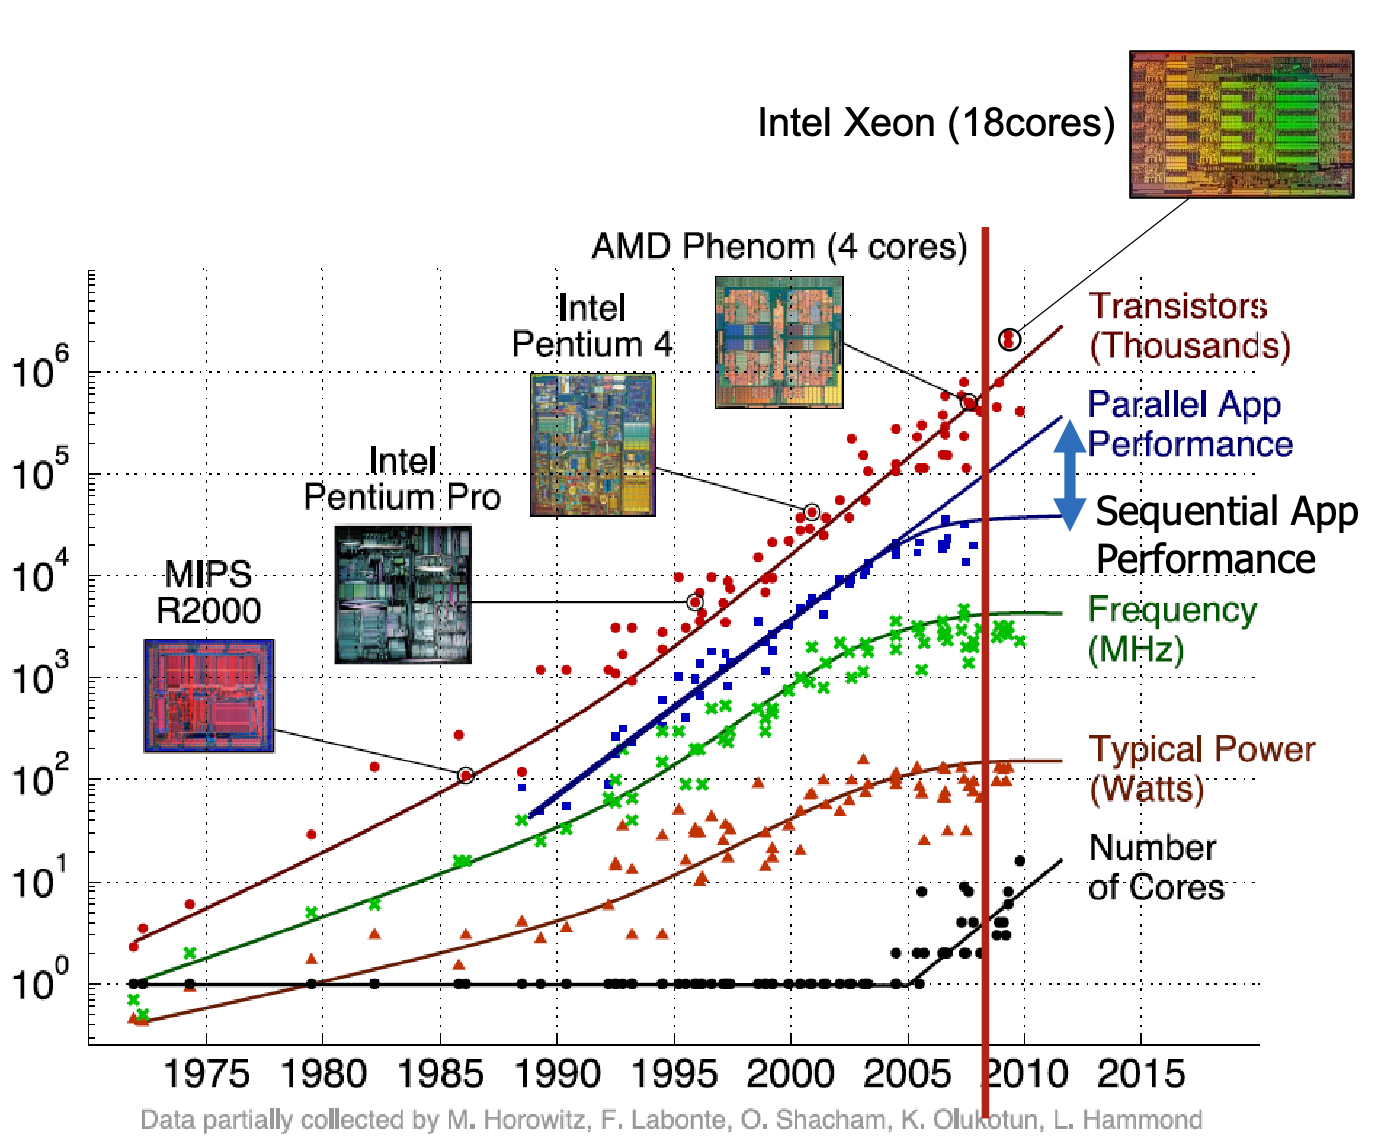
\includegraphics[width=.25\textwidth]{intro_1.png}
\end{wrapfigure}

\noindent$\sim$ 2005: plateau di consumo, frequenza e performance di programmi \textit{sequenziali}, aumento di performance di p.~che \textbf{sfruttano la parallelizzazione} $\rightarrow$ i programmi devono essere "consapevoli" che il processore \`e multicore!\\
Il compilatore mantiene un ruolo fondamentale: oltre a rendere meno "traumatico" il passaggio alla programmazione parallela, (non sono ancora auto-parallelizzanti) si interfaccia con i nuovi paradigmi di programmazione parallela offerti ai programmatori: il programmatore sfrutta interfacce semplici e astratte, mentre il compilatore traduce i costrutti in codice parallelo eseguibile (es. OpenMP)

\subsubsection{Eterogeneit\`a architetturale}

La programmazione parallela e il parallelismo architetturale sono oggi paradigmi consolidati, e i processori general purpose (seppur multicore e ottimizzati) non sono sufficienti per attivit\`a specializzate come la grafica $\rightarrow$ nascono componenti \textbf{acceleratori} di vario tipo: GPU, GPGPU, FPGA, TPU, NPU...
Questo complica ulteriormente la scrittura del software, e dunque impone altre evoluzioni nei compilatori e nelle ottimizzazioni.

\subsection{Ottimizzazione}

Ricordiamo le metriche usate:

\noindent\begin{minipage}[c]{.5\textwidth}
\begin{equation*}
  \text{Performance} = {{1}\over\text{Execution Time}}
\end{equation*}
\end{minipage}
\begin{minipage}[c]{.5\textwidth}
\begin{equation*}
  \text{Execution Time} = {\textcolor{blue}{\text{Instruction Count}} \times \textcolor{red}{\text{CPI}} \over \textcolor{red}{\text{Frequency}}}
\end{equation*}
\end{minipage}\\

Le ottimizzazioni possono avvenire dal punto di vista \textcolor{red}{HW (parametri architetturali)} e da quello \textcolor{blue}{SW (p.~di programma)}. Il compilatore pu\`o agire anche ad es. a livello di cache, aiutando a ridurre i miss e dunque i CPI delle istruzioni \lstinline|load| e \lstinline|store| (sappiamo che il costo di accesso aumenta di ordini di grandezza)

\subsubsection{Esempi di ottimizzazione}

\begin{emphasize}
  Distinguiamo le ottimizzazioni che avvengono a compile time o a runtime (statiche o dinamiche)
\end{emphasize}

\begin{itemize}
  \item \textbf{AS (Algebraic Semplification)}Semplification: ottimizzazione a runtime
  \begin{lstlisting}
-(-i); $\rightarrow$ i;
b or true; $\rightarrow$ true; //cortocircuito logico\end{lstlisting}
  \item \textbf{CF (Constant Folding)}:  valutare ed espandere espressioni costanti a compile time
  \begin{lstlisting}
c = 1+3; $\rightarrow$ c = 4;
(100<0) $\rightarrow$ false\end{lstlisting}
  
  \item \textbf{SR (Strength Reduction)}: sostituisco op. costose con altre pi\`u semplici: classico es. \lstinline|MUL| rimpiazzate da \lstinline|ADD/SHIFT| (esecuzione in 1 ciclo invece di multic.):\\
  \begin{minipage}[c]{.4\textwidth}
  \begin{lstlisting}
y = x*2;
y = x * 17;\end{lstlisting}
  \end{minipage}
  \hfill
  $\rightarrow$
  \hfill
  \begin{minipage}[c]{.4\textwidth}
  \begin{lstlisting}
y = x+x;
y = (x<<4) + x;\end{lstlisting}
  \end{minipage}\\
  es.~sofisticato: \lstinline|for| con operazioni su array, sostituito da operazioni su puntatori (aritmetica dei pt.) $\rightarrow$ il risultato si vede nel codice assembly\\
  \begin{minipage}[c]{.4\textwidth}
  \begin{lstlisting}
for (i=0; i<100; i++)
  a[i] = i*100;
  \end{lstlisting} 
  \end{minipage}
  \hfill
$\rightarrow$
  \hfill
  \begin{minipage}[c]{.4\textwidth}
  \begin{lstlisting}
t = 0;
for (; t<10000; t += 100) {
  *a = t;
  a = a + 4;
}\end{lstlisting}
  \end{minipage}
  
  \begin{minipage}[c]{.4\textwidth}
  \begin{lstlisting}
li s0, 0 // i = 0
li s1, 100
LOOP:
bge s0, s1, EXIT
slli s2, s0, 2
add s2, s2, a0
mul s3, s0, 100
sw s3, 0(s2)
addi s0, s0, 1
jal zero, LOOP
EXIT:\end{lstlisting} 
  \end{minipage}
  \hfill
$\rightarrow$
  \hfill
  \begin{minipage}[c]{.4\textwidth}
  \begin{lstlisting}
li s0, 0 // t = 0
li s1, 10000
LOOP:
bge s0, s1, EXIT
sw s0, 0(a0)
addi a0, a0, 4
jal zero, LOOP
EXIT:\end{lstlisting}
  \end{minipage}
  
\item \textbf{CSE (Common Subexpression Elimination)}: elimino i calcoli ridondanti di una stessa espressione riutilizzata in pi\`u istruzioni (statement)\\
  \begin{minipage}[c]{.4\textwidth}
    \begin{lstlisting}
y = b * c + 4
z = b * c - 1\end{lstlisting}
  \end{minipage}
\hfill $\rightarrow$ \hfill
\begin{minipage}[c]{.4\textwidth}
\begin{lstlisting}
x = b * c
y = x + 4
z = x - 1\end{lstlisting}
\end{minipage}
\item \textbf{DCE (Dead Code Elimination)}: elimino tutte le istruzioni che producono codice mai letto (e dunque utilizzato), es. variabili assegnate e mai lette, codice irraggiungibile $\rightarrow$ uno dei passi eseguiti pi\`u di frequente durante l'ottimizzazione del codice da parte del compilatore, per rimuovere anche tutto il dead code generato dagli altri passi di ottimizzazione\\
  \begin{minipage}[c]{.4\textwidth}
  \begin{lstlisting}
b = 3
c = 1 + 3
d = 3 + c\end{lstlisting}
  \end{minipage}
  \hfill $\rightarrow$ \hfill
  \begin{minipage}[c]{.4\textwidth}
  \begin{lstlisting}
c = 1 + 3
d = 3 + c\end{lstlisting}
  \end{minipage}

  \begin{minipage}[c]{.25\textwidth}
  \begin{lstlisting}
if (100<0)
{a = 5}\end{lstlisting}
  \end{minipage}
  \hfill $\rightarrow$ \hfill
  \begin{minipage}[c]{.25\textwidth}
  \begin{lstlisting}
if (false)
{}\end{lstlisting}
  \end{minipage}
  \hfill $\rightarrow$ \hfill
  \begin{minipage}[c]{.25\textwidth}
  \begin{lstlisting}

  \end{lstlisting}
  \end{minipage}
\item \textbf{Copy Propagation}: per uno statement \lstinline|x = y|, sostituisco gli usi futuri di \lstinline|x| con \lstinline|y| se non sono cambiati nel frattempo (propedeutico alla DCE)\\
  \begin{minipage}[c]{.25\textwidth}
  \begin{lstlisting}
x = y;
c = 1 + x;
d = y + c;\end{lstlisting}
  \end{minipage}
  \hfill $\rightarrow$ \hfill
  \begin{minipage}[c]{.25\textwidth}
  \begin{lstlisting}
x = y;
c = 1 + y;
d = y + c;\end{lstlisting}
  \end{minipage}
  \hfill $\tiny\underrightarrow{\text{DCE}}$ \hfill
  \begin{minipage}[c]{.25\textwidth}
  \begin{lstlisting}
c = 1 + y;
d = y + c;\end{lstlisting}
  \end{minipage}
\item \textbf{CP (Constant Propagation)}: sostituisco usi futuri di una variabile con assegnato valore costante con la costante stessa (se la variabile non cambia) (sempre ipotesi che i valori a fine es.~siano poi \textbf{usati}, e non dead code)\\
  \begin{minipage}[c]{.25\textwidth}
  \begin{lstlisting}
b = 3;
c = 1 + b;
d = b + c;\end{lstlisting}
  \end{minipage}
  \hfill $\tiny\underrightarrow{\text{CP}}$ \hfill
  \begin{minipage}[c]{.25\textwidth}
  \begin{lstlisting}
b = 3;
c = 1 + 3;
d = 3 + c;\end{lstlisting}
  \end{minipage}
  \hfill $\tiny\underrightarrow{\text{CF}}$ \hfill
  \begin{minipage}[c]{.25\textwidth}
  \begin{lstlisting}
b = 3;
c = 4;
d = 3 + c;\end{lstlisting}
  \end{minipage}
  \hfill $\tiny\underrightarrow{\text{CP}}$ \hfill

  \hfill $\tiny\underrightarrow{\text{CP}}$ \hfill
  \begin{minipage}[c]{.25\textwidth}
  \begin{lstlisting}
b = 3;
c = 4;
d = 3 + 4;\end{lstlisting}
  \end{minipage}
  \hfill $\tiny\underrightarrow{\text{CF}}$ \hfill
  \begin{minipage}[c]{.25\textwidth}
  \begin{lstlisting}
b = 3;
c = 4;
d = 7;\end{lstlisting}
  \end{minipage}
  \hfill $\tiny\underrightarrow{\text{DCE}}$ \hfill
  \begin{minipage}[c]{.25\textwidth}
  \begin{lstlisting}
d = 7;\end{lstlisting}
  \end{minipage}
\item LICM (Loop Invariant Code Motion): si occupa di muovere fuori dai loop tutto il codice \textbf{loop invariant}; evita i calcoli ridondanti\\
  \begin{minipage}[c]{.4\textwidth}
  \begin{lstlisting}
while (i<100) {
  *p = x/y + i;
  i = i + 1;
}\end{lstlisting}
  \end{minipage}
  \hfill $\rightarrow$ \hfill
  \begin{minipage}[c]{.4\textwidth}
  \begin{lstlisting}
t = x + y;
while (i < 100) {
  *p = t + i;
  i = i + 1;
}\end{lstlisting}
  \end{minipage}
\end{itemize}

\subsubsection{Ottimizzazioni sui loop}

\begin{itemize}
  \item grande impatto sulla performance dell'intero programma (per ovvie ragioni)
  \item spesso sono ottimizzazioni propedeutiche a quelle machine-specific (effettuate nel backend): register allocation, instruction level parallelism, data parallelism, data-cache locality
\end{itemize}

\subsection{Anatomia di un compilatore}

\begin{figure}[h]
  \centering
  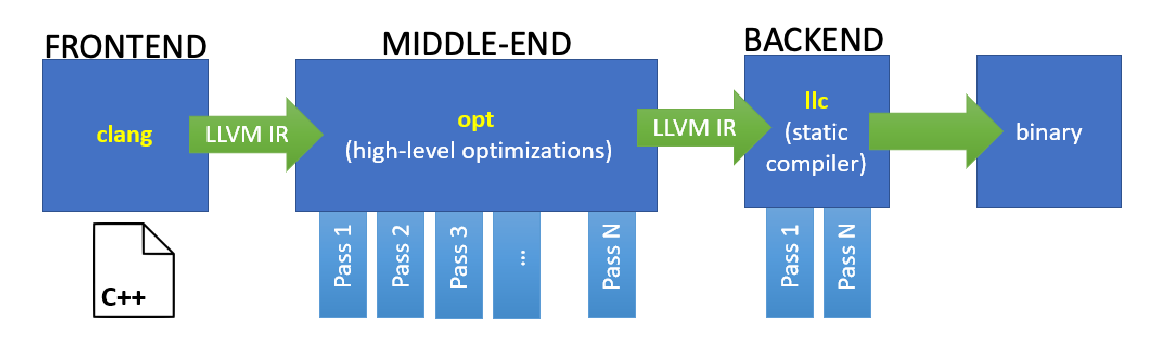
\includegraphics[width=.5\textwidth]{intro_3.png}
\end{figure}

\begin{itemize}
  \item almeno due compiti: \textbf{analisi del sorgente} e \textbf{sintesi di un programma in linguaggio macchina}, operando su una IR che si interpone tra frontend e backend, e tra source code e target code
  \item Il blocco di middle-end agisce su IR, e in vari passaggi lo trasforma e ottimizza ($\neq$ a seconda del compilatore)
  \item caso llvm: \lstinline|clang| (frontend) $\rightarrow$ \lstinline|opt| (middleend) $\rightarrow$ \lstinline|llc| (backend)
  \item \lstinline|opt| si basa su una serie di \textbf{passi di ottimizzazione (o di analisi)}: un passo di analisi scorre l'IR e lo analizza (non lo trasforma, ma produce informazioni utili); un passo di ottimizzazione sfrutta informazioni conosciute per trasformare l'IR (applica le ottimizzazione)
  \item alcune ottimizzazioni non possono essere effettuate o finalizzate senza conoscere l'architettura target (es. sulle cache), e dunque vengono eseguite dal backend
\end{itemize}

\subsubsection{Flag di ottimizzazione}

sono flag che passo al compilatore (al pass manager) per influenzare \textbf{ordine e numero dei passi di ottimizzazione}
\begin{multicols}{2}
\begin{itemize}
  \item \lstinline|-g|: solo debugging, nessuna ottimizzazione
  \item \lstinline|-O0|: nessuna ottimizzazione
  \item \lstinline|-O1|: solo ott. semplici
  \item \lstinline|-O2|: ott. pi\`u aggressive
  \item \lstinline|-O3|: ordine dei passi che sfrutta compromessi tra velocit\`a e spazio occupato
  \item \lstinline|-OS|: ottimizza per dimensione del compilato
\end{itemize}
\end{multicols}


\subsubsection{Uso di IR}

un backend che fa uso di IR permette di disaccoppiare con facilit\`a frontend e backend, lavorare su ottimizzazioni machine-independent, semplificare il supporto per molti linguaggi, eccetera

\begin{emphasize}
  Per supportare un nuovo linguaggio o una nuova architettura, basta scrivere un nuovo front/backend - il middle-end pu\`o rimanere lo stesso!
\end{emphasize}

\subsubsection{Ingredienti dell'ottimizzazione}

\begin{itemize}
  \item \textbf{formulare un problema di ottimizzazione} con molti casi di applicazione, sufficientemente efficiente e impattante su parti significative
  \item[$\rightarrow$] \textbf{rappresentazione} che astrae dettagli rilevanti $\rightarrow$ \textbf{analisi} di applicabilit\`a $\rightarrow$ \textbf{trasformazione del codice} $\rightarrow$ \textbf{testing} $\rightarrow \, \circlearrowleft$
\end{itemize}

\vspace{-2em}
\section{Rappresentazione intermedia (4 mar)}

Ricordiamo: middle end come sequenza di passi, di analisi o di trasformazione $\rightarrow$ per analizzare e trasformare il codice occorre una rappr.~intermedia (IR) \textbf{espressiva} che \textbf{mantenga le informazioni importanti da un passo all'altro}

\vspace{-1em}
\subsection{Propriet\`a di una IR}

scegliamo IR diverse a seconda del loro uso, in generale alcune caratteristiche sono sempre richieste:
\begin{itemize}
  \item facilit\`a di \textbf{generazione} (effetti sul frontend)
  \item facilit\`a e costo di \textbf{manipolazione}
  \item livello di astrazione e di \textbf{dettaglio esposto}: effetti su frontend e backend ($\neq$ IR da un lato e dall'altro, a seconda di astraz.~e dettaglio necessari)
\end{itemize}

\vspace{-1em}
\subsection{Tipi di IR}

\begin{itemize}
  \item AST (abstract syntax tree)
  \item DAG (grafi diretti aciclici)
  \item 3AC (3-address code): simile all'assembly (3 indirizzi: registro destinazione e max 2 operandi)
  \item SSA (Static Single Assignment): evoluzione di 3ac con ulteriori propriet\`a di control flow
  \item CFG (control flow graphs): rappresenta "come" vengono chiamate le funzioni (a partire dal main)
  \item CG (call graph)
  \item PDG (program dependence graphs): fondamentale per lavorare sul parallelismo, multithreading...
\end{itemize}

\vspace{-1em}
\begin{emphasize}
  Le ott.~inter-procedurali devono per forza basarsi su IR di tipo CG (es. per decidere quando fare \textbf{inlining} - espandere il codice della funzione invece di chiamarla - evidente tradeoff tra dimensione del codice e overhead dovuto alla chiamata di funzione)
\end{emphasize}

\subsection{Categorie di IR}

\begin{itemize}
  \item grafiche (o strutturali)
    \begin{itemize}
      \item orientate ai grafi
      \item molto usate nella source-to-source translation, tipicam.~per ott.~che non hanno bisogno della struttura sofisticata di un middle-end\\
      es.~openMP: di fatto annotazioni sul codice, come strumento semplice per la parall.~(es. \textbf{outlining}: prendo es un loop e lo impacchetto in una funzione che poi dovra essere eseguita dai thread per la parallelizzazione) - non sto ottimizzando nel senso proprio del termine, ma sto trasformando il codice e lo sto rendendo eseguibile in maniera parallela
      \item solitamente voluminose (basate su grafi) - tradeoff con il fatto che non coinvolgono il middle-end
      \item es. ast, dag
    \end{itemize}
  \item lineari
    \begin{itemize}
      \item pseudocodice per macchine astratte
      \item livello di astrazione vario
      \item strutture dati semplici e compatte
      \item facile da riarrangiare (evidentemente il pi\`u comodo per eseguire le ottimizzazioni)
      \item es. 3ac
    \end{itemize}
  \item ibride (sfruttano combinazioni delle prime due) (es cfg)
\end{itemize}
\subsection{Esempi di rappresentazione}


\subsubsection{Sintassi concreta (testo)}

Pi\`u semplice in quanto pi\`u vicina al livello di astrazione "umano" di ragionamento sul programma, ma non il livello corretto per ottimizzare ne comprendere correttamente la semantica del programma

\begin{lstlisting}[language=java]
let value = 8;
let result = 1;
for (let i = value; i>0; i = i - 1) {
  result = result * i;
}
console.log(result);\end{lstlisting}

\vspace{-.5em}
\subsubsection{AST}

Albero i cui nodi rappresentano diverse parti del programma: il nodo radice rappresenta il \textbf{programma}, il quale a sua volta contiene un blocco di istruzioni dal quale discendono tanti figli quante le sue istruzioni

\noindent\begin{minipage}[c]{.3\textwidth}
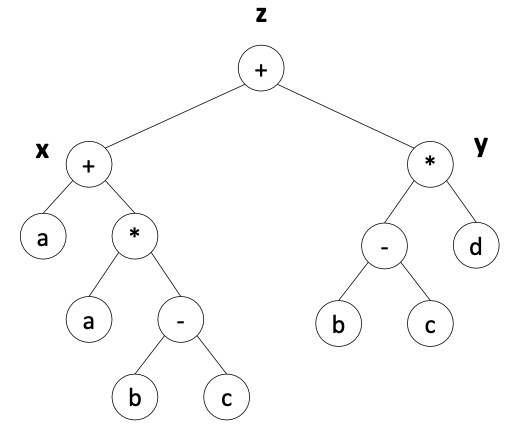
\includegraphics[width=\textwidth]{ir_1.png}
\end{minipage}
\begin{minipage}[c]{.7\textwidth}
\begin{lstlisting}
x = a + a * (b - c)
y = (b - c ) * d
z = x + y\end{lstlisting}
\textbf{PRO}: molto comodo per interpreti (basta usare una fz.~ricorsiva per processare l'albero)

\textbf{CONTRO}: un nodo \`e un oggetto troppo generico $\rightarrow$ analizzare un ast per l'ottimizzazione impone ogni volta di ragionare sulla differenza semantica tra i nodi (complica molto)
\end{minipage}


\vspace{-.5em}
\subsubsection{DAG}

Contrazione di ast che evita la duplicazione di espressioni $\rightarrow$ \textbf{rappresentazione pi\`u compatta}

\noindent\textbf{Limite}: il riuso e possibile solamente dimostrando che il suo \textbf{valore non cambia} nel programma
\begin{emphasize}
  essendo assegnamenti e chiamate frequentissimi, il fatto che il dag non abbia nozione di come le espr.~cambino valore nel tempo non lo rende un buon candidato per le ottimizzazioni
\end{emphasize}

\begin{example}[frametitle={Esempi}]
   \noindent\begin{minipage}[c]{.2\textwidth}
   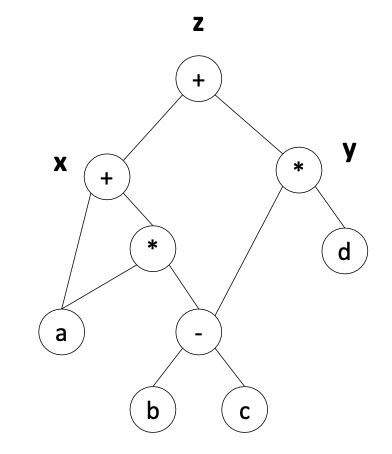
\includegraphics[width=\textwidth]{ir_2.png}
   \end{minipage}
   \begin{minipage}[c]{.23\textwidth}
      \begin{lstlisting}
x = a+a*(b-c);
y = (b-c)*d;
z = x+y;
# espr. trovate
t1 = b-c;
t2 = a*t1;
x = a+t2;
y = t1*d;
z = x+y;\end{lstlisting}
   \end{minipage}\hfill\vline
   \begin{minipage}[c]{.2\textwidth}
   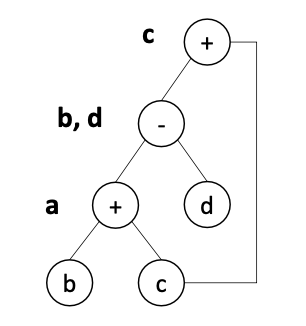
\includegraphics[width=\textwidth]{ir_3.png}
   \end{minipage}
   \begin{minipage}[c]{.35\textwidth}
      \begin{lstlisting}
a = b + c;
b = a - d;
c = b + c;
d = a - d;
# espr. trovate (ERRORE)
a = b + c; # cambia val.
d = a - d;
c = d + c;\end{lstlisting}
   \end{minipage}
\end{example}



\subsubsection{3AC}


\begin{minipage}[c]{.65\textwidth}
Evidentemente adatto: tutte le istr.~del programma vengono spezzettate in istr.~di forma semplice simile all'assembly, di tipo \lstinline|x = y op z| (1 operatore, massimo 3 operandi)

\noindent
  \begin{minipage}[c]{.3\textwidth}
    \begin{lstlisting}
x - 2 * y\end{lstlisting}
  \end{minipage}
  $\rightarrow$
  \begin{minipage}[c]{.32\textwidth}
    \begin{lstlisting}
t1 = 2 * y
t2 = x - t1\end{lstlisting}
  \end{minipage}
\end{minipage}
  \hfill
  \begin{minipage}[c]{.3\textwidth}
  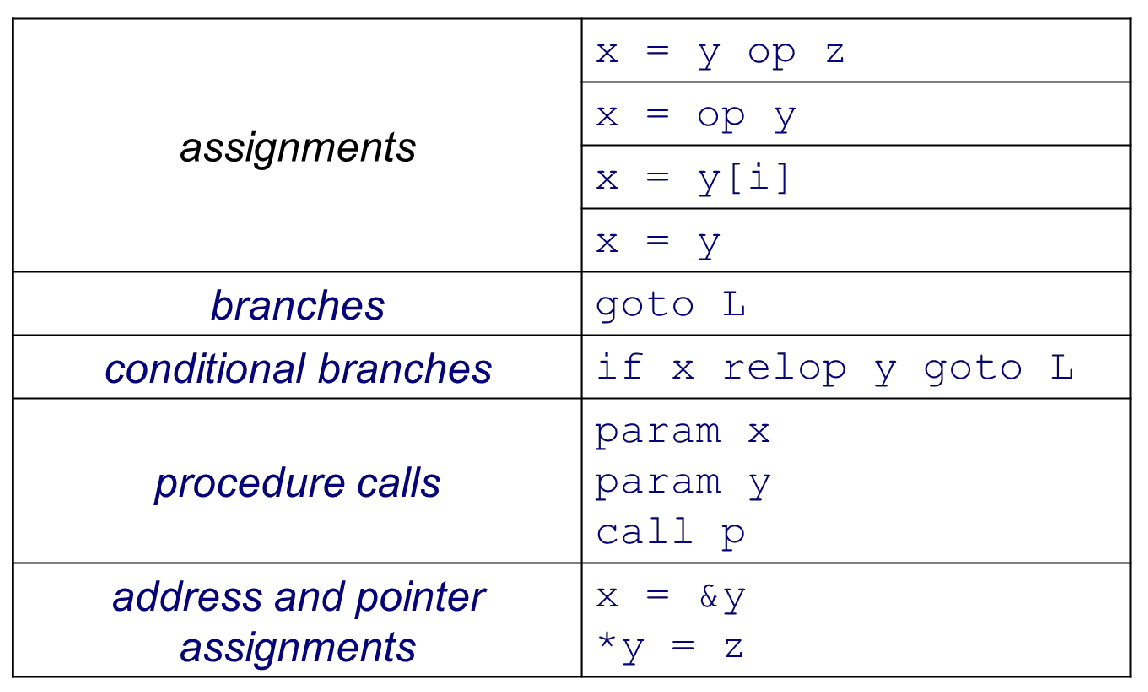
\includegraphics[width=\textwidth]{ir_4.png}
  \end{minipage}

\textbf{PRO}:
\begin{itemize}
  \item espressioni complesse spezzettate
  \item forma compatta e simil-assembly
  \item registri temporanei \textbf{intermedi, virtuali e illimitati} (tralascio problemi architetturali - n.~di r.~fisici a disposizione e eventuali op. di spill, cio\`e aggiungere load o store in mancanza di r.~fisici)
\end{itemize}

\paragraph{Varianti di 3AC}~\\

A seconda dei vincoli che ho per l'implementazione pratica:

\begin{itemize}
  \item quadruple: id istruzione, opcode, i 3 registri $\rightarrow$ semplice struttura record, facile da analizzare e riordinare ma i nomi espliciti prendono pi\`u spazio
  \item triple: id istruzione, opcode, 2 operandi $\rightarrow$ uso l'indice dell'espressione nell'array come "nome" del registro destinazione $\rightarrow$ risparmio spazio, ma diventa piu complesso da analizzare (nomi impliciti) e riordinare
\end{itemize}


Ricordiamo la constant propagation: sostituisco usi futuri di una variabile con valore costante con la costante stessa \textbf{se non cambia nel frattempo}

$\rightarrow$ ottimizzazione che una IR di tipo 3ac non puo applicare immediatamente (devo prima analizzare il resto del codice) $\rightarrow$ SSA come evoluzione della 3ac, in quanto impone che la \textbf{definizione (assegnamento)} delle variabili avvenga \textbf{solo una volta} (definizioni multiple sono tradotte in multiple versioni della var)

pro: ogni definizione ha associata direttamente una lista di tutti i suoi usi - semplifica enormemente le ottimizzazioni di tipo CP e non solo

quasi sempre uno dei passi di ottimizzazione prevede il passaggio a forma SSA

\begin{emphasize}
  La scelta della IR dipende ovviamente dal livello di dettaglio necessario per ogni specifico compito $\rightarrow$ \textbf{in un compilatore coesistono pi\`u IR}

  \noindent Anche per questo ci sono le forme ibride - es. cfg con 3ac
\end{emphasize}

\subsubsection{cfg}

vediamo un esempio con costrutti condizionali (non solo sequenze lineari)

immagine slide 2-28

un cfg permette di aggiungere informazioni sui \textbf{salti} al di sopra di una IR lineare $\rightarrow$ modello il flusso di controllo del programma come grafo composto da blocchi (BB)

ogni bb contiene sequenze lineari di istruzioni

gli archi rappresentano il flusso di controllo del programma


formalmente: un BB \`e una seq.~di istruzioni in forma 3AC
\begin{itemize}
  \item solo la prima istruzione puo essere raggiunta dall'esterno (garantito un singolo entry point)
  \item singolo exit point: se eseguo la prima istr.~\textbf{devo eseguire tutte le altre} - garantisco che venga eseguito interamente
\end{itemize}

le chiamiamo sezioni single-entry, single-exit (possono essere sezioni anche piu grandi, ma le piu piccole di questo tipo sono i BB)

un arco connette due nodi s.s.se il secondo puo eseguire dopo il primo in qualche percorso del ctrl flow del programma (prima istr del secondo \`e target dell'istr di salto al termine del primo, oppure il secondo \`e l'unico successore del primo che non ha un istr di salto come ultima istr - il secondo lo chiamo nodo falltrough)

un cfg \textbf{normalizzato} ha i bb \textbf{massimali} (non possono essere resi piu grandi senza violare condizioni) (unisco i bb fallthrough che non hanno label all'inizio, evidentemente) (situazioni di cfg non normalizzato possono avvenire dopo qualche generico passo di ottimizzazione, evidentemente non le facciamo accadere noi "spontaneamente")

\paragraph{algoritmo per la costruzione del cfg}~\\

\begin{enumerate}
  \item identificare il \textbf{leader} di ogni bb:
    \begin{itemize}
      \item la prima istruzione
      \item il target di un salto
      \item ogni istruzione dopo un salto
    \end{itemize}
  \item il bb comincia con il leader e termina con l'istruzione immediatamente precedente un nuovo leader (o l'ultima istruzione)
  \item connettere i bb tramite archi di 3 tipi:
    \begin{itemize}
      \item fallthrough (o fallthru): esiste solo un percorso che collega i due blocchi
      \item true: il secondo blocco \`e raggiungibile dal primo se un condizionale \`e true
      \item false: il secondo blocco \`e raggiungibile dal primo se un condizionale \`e false
    \end{itemize}
    
\end{enumerate}

esempi ed esercizi fino slide 52

\subsubsection{dependency graph}

soprattutto nell'erad ei nulticore questa rappr assume sempre piu importanza

almeno due tipi: (recupera questa cosa)

ricordiamo pipeline riscv e data hazard: il fatto che un registro voglia leggere da un registro usato in un'op precedente (e non ancora salvato? recupera)

if id exe mem wb le fasi di pipelining

esempio con una mul: ricordiamo che se la mul successiva prova a usare il registro usato nell'istr prima (dipendenza), il risultato ancora non e stato scritto - nella fase di decode identifico i registri usati nell'operazione, e appunto rw ancora non contiene il risultato aggiornato, che sara pronto appena tra 2 cicli

questo e un data hazard, nel caso comune si gestisce con una \textbf{forwarding unit} che bypassa le fasi successive e inoltra direttamente il risultato appena ottenuto

per quanto la fw unit sia un pezzo di hw dedicato che fa questi controlli autonomamente, in generale l'unico modo per evitare questo tipo di hazard \`e distanziare abbastanza le istruzioni tra loro affinche il dato sia disponibile $\rightarrow$ sposto l'istruzione di mul inserendo nop (cicli di stallo) (evidentemente non buono - vado a "rompere" l'IPC paria a 1 della pipeline sempre piena, evidentemente diminuisce la performance)

soluzione migliore: scheduling del programma, ovvero sposto istruzioni che non hanno bisogno di quei registri per riempire quello spazio altrimenti occupato necessariamente da nop

questo \`e uno dei compiti principali di un backend - \textbf{in che ordine genero le istruzioni per massimizzare l'efficienza del programma}

come faccio a fare questa cosa? manualmente: vado a guardare le istruzioni e cerco a mano le dipendenze; il backend sfrutta la IR di tipo dg che fornisce esattamente le informazioni sulle dipendenze tra istruzioni

qui si capisce cosa si intende per instruction level parallelism: dunque, quando \`e possibile sfruttare tutte le parti di architettura per "parallelizzare il codice" anche in caso di single thread (ottimizzazione senza reale parallelismo)


\subsubsection{data dependency graph ddg}

Specifico per multicore e parallelismo, usato per dare una rappresentazione tra le dipendenze dei \textbf{dati} - tipicamente i loop

per esempio, (loop innestati lavorano tipicamente su str dati complesse e multidimensionali (matrici, immagini, ecc.))

\begin{lstlisting}
for (i = 0, i < n, i++)
  A[i]=init();
\end{lstlisting}


Ogni it. resta indipendente dalle altre (uso il solo indice del loop) - basta aggiungere ad es.~ \lstinline|A[i-1] = A[i]| per generare dipendenze tra le iterazioni $\rightarrow$ il loop non \`e pi\`u parallelizzabile, e deve per forza essere eseguito in sequenza

Data la complessit\`a delle casistiche reali,  esistono vari modi per rappresentare lo spazio delle iterazioni di un loop e le dipendenze che ne derivano:\\
all'oggi usiamo il \textbf{polyhedral model} $\rightarrow$ rappresento lo spazio delle it.~come un poliedro (a seconda del numero di loop innestati), che permette di capire se esiste qualche permutazione dei loop (direzione di attraversamento dello spazio delle iterazioni; ovvero ad esempio scambiare l'ordine dei loop) non soggetta a dipendenze

\subsubsection{call graph}

rappresetnazione grafica a grafo usata per ragionare sulle relazione tra le funzioni della translation unit del file (insieme delle potenziali chiamate tra funzioni)

rappr.~gerarchica, utile soprattutto a livello di analisi \textbf{interprocedurale} (la maggior parte delle ottimizzazioni avvengono a livello \textit{intraprocedurale}) (recupera questo concetto) (lavora sui file che abbiamo chiamato translation units, ovvero quelli da cui poi genero i file oggetto)

$\rightarrow$ evidente come il compilatore abbia visibilita solo fino a livello dei singoli moduli: posso estendere le ottimizzazioni al massimo fino ai legami tra funzioni dello stesso modulo - le ottimizzazioni piu ampie si spostano a framework di ottimizzazione che agiscono a livello di linker per esempio

\section{Ottimizzazione locale e basic value numbering - 24 marzo}

\subsection{scope dell'ottimizzazione}

finora abbiamo lavorato in locale, ovvero all'interno di un singolo BB $\rightarrow$ un'ott.~locale non si preoccupa del flusso di controllo di un programma, mentre una globale lavora a livello dell'intero CFG $\rightarrow$ lo scope viene influenzato da come viene gestito il flusso di controllo in un programma

\begin{itemize}
  \item ott locale: entro un sibgolo bb, non si preoccupa del flusso
  \item ott globale: lavora a livello dell'intero CFG
  \item ott interprocedurale: lavora a livello del call graph, e quindi sui CFG di pi\`u funzioni
\end{itemize}

\begin{example}[frametitle={dead code elimination}]
  es di ott locale
  \begin{lstlisting}
main {
  int a = 4;
  int b = 2;
  int c = 1;
  int d = a + b;
  print d;
}\end{lstlisting}
 evidentemente dobbiamo togliere la def di c, ma: solo quello? ricorda che rappresentano dead code le istr che definiscono (assegnano un valore a) una var che non \`e mai utilizzata $\rightarrow$ poiche la print non definisce nulla, stando a questa def \`e dead code! invece, estendiamo la definizione dicendo che lo sono le istr \textbf{prive di side effects} che definiscono ... 


  proviamo a costruire un algoritmo per implementare la dce cos\`i definita:
  \begin{enumerate}
    \item $\forall$ istruzione in BB
    \begin{itemize}
      \item aggiungi operandi ad un metadato array \lstinline|used|
    \end{itemize}
    \item $\forall$ istr in BB
    \begin{itemize}
      \item se istr non ha destinazione e non ha side effects rimuovila
      \item altrimenti se la destinazione non corrisponde a nessuno degli elem di \lstinline|used| rimuovila
    \end{itemize} 
  \end{enumerate}

  dall'esempio vediamo che funziona, ma iterativamente potremmo eliminare poi altre istr $\rightarrow$ soluzione semplice \`e aggiungere la parte iterativa all'algoritmo, che dunque esegue fino a convergenza
  
\end{example}

\begin{example}
    altro esempio: ridefinizione di una variabile (slide 6-22) - ovvero il nostro algoritmo corrente non gestisce le dead stores

    \begin{emphasize}
      in generale, capiamo che scrivere un passo significa prima definire bene cosa deve fare...
    \end{emphasize}
    
    per estendere l'algoritmo, dobbiamo essere in grado di rilevare gli assegnamenti multipli di una variabile, e quindi anche preoccuparci dell'ordine delle istruzioni! (pi\`u complicato)

    analizzando pseudocodice a 6-29: lista di variabili definite; itero sulle istruzioni e rimuovo gli operandi da \lstinline|last_def| (sono variabili usate da qualche parte) ; poi controllo le definizioni: se la destinazione dell'istruzione (LHS) si trova ancora in lastdef, la elimino da li e al suo posto metto l'istruzione stessa (??????????) (vedi da 6-29 a 6-38 per spiegazione iterativa fatta benino)
\end{example}

\subsection{Local value numbering}

tecnica utilizzata per considerare il concetto di ordine delle definizioni in assenza di propriet\`a di tipo SSA (che ti permette di non avere questo problema)

osserviamo 3 pattern che forniscono opportunit\`a di eliminazione di codice ridondante:
\begin{itemize}
  \item dead code elimination: 1 variabile e piu valori
  \item copy propagation: 1 valore e piu variabili
  \item common subexpression elimination: 1 valore (in forma di espressione) e piu variabili
\end{itemize}

\begin{lstlisting}
main {
  int a = 100;
  int a = 42;
  print a;
}\end{lstlisting}

\begin{lstlisting}
main {
  int x = 4;
  int copy1 = x;
  int copy2 = copy1;
  int copy3 = copy2;
  print copy3;
}\end{lstlisting}

\begin{lstlisting}
main {
  int a = 4;
  int b = 2;
  int sum1 = a + b;
  int sum2 = a + b;
  int prod = sum1 * sum2;
  print prod;
}\end{lstlisting}

sono tutti modelli di computazione che si focalizzano sulle \textbf{variabili} $\rightarrow$ focalizzandoci sui \textbf{valori} possiamo eliminare tutte le forme di ridondanza

soluzione ai tempi in cui ancora non era in uso il modello ssa: local value numbering

tecnica che ci aiuta nelle ott.~proprio per il cambio focus da variabili a valori

costruisco un metadato in forma di tabella che riscrive le espr (istruzioni) in funzione dei valori gia osservati $\rightarrow$ evitando di riassegnare lo stesso valore a piu var si evita la ridondanza

esempio da 6-46 a 6-56

analizzo le istruzioni in termini del value, e in caso questo coincida con entry della tabella gia presenti punto direttamente a quella

semplice variante del programma:
\begin{lstlisting}
#...
int sum1 = a + b;
int sum2 = b + a;\end{lstlisting}

evidentemente nascono problemi, poiche il nostro algoritmo non conosce le proprieta aritmetiche delle operazioni $\rightarrow$ non vado a rimuovere l'istruzione

$\rightarrow$ soluzione semplice: \textbf{canonicalizzare} l'algoritmo, ovvero imporre un ordine numerico tra le entry (i valori) e usarle sempre in ordine crescente per le op. commutative (di fatto \`e la tecnica usata da tutti i compilatori, essendo al piu semplice?)

\section{data flow analysis}

step successivo dell'analisi, da immaginare come un framework di analisi alla base per costruire la forma ssa (?) ; o come una metodologia di analisi

\subsection{cos'\`e la dfa}

\begin{itemize}
  \item analisi locale: si focalizza sull'effetto di ogni istruzione $\rightarrow$ posso comporre gli effetti di tutte el istr per derivare informazione dall'inizio del bb ad ogni istruzione
  \item analisi globale - dataflowanalysis: simile, ma molto pi\`u complessa $\rightarrow$ analizza l'effetto di ogni BB, e poi ha una metodologia per comporre l'effetto dei BB ai CONFINI degli stessi per derivare informazione
\end{itemize}

skip 7-6

esempio 7-7 struttura ad amaca (hammock) - statement di tipo if che dirama su due possibili flussi di controllo $\rightarrow$ per ogni variabile x consente di derivare
\begin{itemize}
  \item valore di x?
  \item quale "definizione" definisce x?
  \item la definizione \`e ancora valida (\textit{live})?
\end{itemize}

osserviamo che queste risposte noi le abbiamo gia ottenute in maniera molto semplice, grazie alla forma SSA delle istruzioni! e alla struttura di llvm

nota: stiamo "costruendo" la forma SSA, considerando un caso in cui non abbiamo ancora quel liverllo?

\subsection{rappresentazione del programma statica o dinamica}

statica: programma finito, un pezzo di codice $\rightarrow$ molto facile da analizzare
dinamica: pu\`o avere infiniti percorsi di esecuzione, rappresenta una possibile esecuzione reale! $\rightarrow$ es. loop che si basa sull'analisi di un input

sono condizioni che un compilatore non pu\`o analizzare, soprattutto non in maniera statica e "finita" in termini di possibili istanze

\begin{emphasize}
    capacita di analisi dei compilatori: limitata alle condizioni analizzabili e determinabili \textbf{staticamente}

    motivo per cui spesso si passano al compilatore informazioni di "profiling" , misurate durante ripetute esecuzioni del programma prima di darlo in pasto al compilatore e i relativi passi di ottimizzazione
\end{emphasize}

con la dfa siamo in grado di dire \textbf{per ogni punto del programma} qualcosa; combinando informazioni relative a tutte le possibili istanze dello stesso p.to

esempio di problema dfa: quale def definisce il valore usato nello statement \lstinline|b=a|? vedi da slide 7-8 il codice

\subsubsection{effetti di un bb}

effetti di un'istruzione:
\begin{itemize}
  \item uses : delle variabili
  \item kills : una precedente definizione
  \item defines : una variabile
\end{itemize}
combinando gli effetti delle singole istr si definiscono gli effetti di un BB:
\begin{itemize}
  \item uso localmente esposto (locally exposed use): in un bb \`e un uso di una var che non \`e preceduto nei bb da una definizione della stessa variabile
  \item ogni definizione di una variabile nel BB killa tutte le definizioni delal stessa variabile che \textbf{raggiungono} il BB
  \item definizione localmente disponibile (locally available definition): ultima definizione di una variabile nel bb
\end{itemize}

esempio: 7-15

\subsubsection{reaching definition}

ogni istruzione di assegnamento \`e una definizione
una definizione \textit{d} raggiunge (reaches) un punto it\textit{p} se esiste un percorso da \textit{d} a \textit{p} tale per chu d non \`e uccisa (sovrascritta) lungo quel percorso

definizione del problema: determinare per ogni punto del programma se ogni definizione nel programma raggiunge quel punto - come lo facciamo? $\rightarrow$ usiamo un \textbf{bit vector} per ciascun punto del programma (ogni istruzione), con lunghezza del vettore pari al numero di definizioni $\Rightarrow$ diventa una sorta di matrice con righe le istruzioni, colonne le definizioni

\subsubsection{schema dfa}

consideriamo un flow graph che ha sempre un BB entry e uno exit (single-entry e single-exit $\rightarrow$ sempre possibile)

come faccio a stabilire l'effetto del codice in ciascun BB? uso quelle che si chiamano funzioni di trasferimento: fz che correlano input e output tra loro per un dato bb

qual \`e l'effetto del flusso di controllo? lo stabilisco in base alla vicinanza dei blocchi: correlo outp e inp di blocchi adiacenti

alla fine dobbiamo solo risolvere queste equazioni 

\subsubsection{effetti di uno statement}

partiamo dalle fz di trasf di statement (astrazione per indicare un istr? di assegnamento?)

l'output di uno statement ... rec blabla

ricorda che stiamo lavorando su bit vector!!!!!!!!!!!!!! una fz di trasferimento riempie out[s] a partire da in[s] e applicando qualche tipo di calcolo

alla fine posso combinare queste funzioni di trasferimento in maniera lineare! (non lo dim ma si potrebbe)

quindi la funz di tr di un BB compone linearmente le fz dei suoi statements

rec da carta e slide

\subsubsection{effetti degli archi aciclici}

caso predecessori multipli: unisco l'informazione con che criterio? join

oggi fino slide 7-42

ricordiamo che in generale stiamo usando un "approccio" bit-vector, che non possiede nozione di ordine di esecuzione - quando calcolo i kill, li calcolo sempre relativamente a \textbf{tutti gli altri blocchi!} es. slide 7-36: $Kill[B_1] = \left\lbrace0,2,3,4,6\right\rbrace$

riprendiamo la questione sugli effetti degli archi aciclici, nel caso di un nodo con predecessori multipli:
\begin{itemize}
  \item $out[b] = f_b(in[b])$
  \item nodo di unione (join): nodo con predecessori multipli
  \item operatore di unione (meet): $in[b] = out[p_1] \cap out[p_2] \cap \ldots \cap out[p_n]$ con $p_1,\ldots,p_n$ tutti predecessori di $b$
  \item caso entry block: $out[\text{entry}] = \emptyset \implies in[B_1] = \emptyset$ \textbf{boundary condition}
  \item caso exit dall'esempio: $in[\text{entry}] = out[B_2] \cap out[B_3] = \lbrace 2,3,4,5,6 \rbrace$
\end{itemize}

notiamo come i due modi (bit-vector oppure usare join e meet) sono equivalenti (?)

\subsubsection{effetti degli archi ciclici}

notiamo un problema con gli archi \textbf{ciclici} - posso arrivare a condizioni in cui non ho ancora calcolato l'out di un qualche bb, ma mi serve per un arco ciclico appunto che punta a un blocco precedente

soluzione: devo iterare fino a convergenza, ma soprattutto definire delle condizioni iniziali (come per l'out dell'entry block) che ci dicono che in uscita ad ogni blocco (all'inizio) trovo l'insieme vuoto (necessaria per avere qualcosa su cui operare alla prima iterazione che considera dei backedge)

\subsection{liveness analysis}

\subsubsection{live variable analysis}

definizioni: variabile live o dead: una var \`e viva in un punto p del programma se il valore di v \`e usato da quel punto in avanti da qualche parte nel programma - altrimenti \`e morta

altri possibili motivi di questa analisi (oltre alla dce): register allocation: nel momento in cui devo fare i conti con un'architettura specifica, devo decidere come allocare i registri (non sono illimitati) - register allocation \`e l'op.~che cerca di evitare le spill in cache e in memoria, e che cerca i casi in cui risulta possibile riutilizzare un certo registro: dipende evidentemente dalla liveness di una variabile!

definizione del problema in termini di dfa: $\forall$ BB devo stabilire se ogni variabile \`e viva in ciascuno di essi $\rightarrow$ bit vector di lunghezza pari al numero di variabili (evidentemente...)

\subsubsection{funzione di trasferimento}

recupera questione su forward analysis

che informazione sto cercando per capire se una definizione raggiunge o meno un punto del programma? devo analizzare "il passato" - gli statement tra la definizione e il punto di interesse per cercare eventuali kill (analizzo dal punto all'entry point, a ritroso)

nel contesto della liveness analysis invece, devo analizzare il "futuro" - dal punto p all'exit point cerco gli usi della variabile

(abbiamo spiegato la differenza tra forward e backward analysis, nelle sezioni prima abbiamo implicitamente considerato backward analysis per il problema di reaching definition)

per la formulazione pi\`u tipica della liveness analysis (ce ne sono diverse, a seconda delle fonti) usiamo
\begin{itemize}
  \item l'insieme delle variabili vive che pu\`o generare un BB (use)
  \item l'insieme delle variabili definite nel BB (def)
  \item le variabili vive in ingresso che il bb pu\`o propagare (out - def)
  \item fz di trasferimento quindi \`e: in = use U out - def
\end{itemize}

\begin{emphasize}
    nota che di fatto stiamo riscrivendo quello che abbiamo detto per la reaching definition! solo al contrario - in questo momento stiamo risalendo al contrario per calcolare gli insiemi che ci servono e le funzioni di trasferimento, e sarebbe sufficiente "sostituire" come nomenclatura use e def con gen e kill (non mi ricordo se questo \`e l'ordine giusto)
\end{emphasize}

anche qui abbiamo quindi un operatore di meet, applicabile ai join node (nodi con \textbf{successori} multipli)

esempio 7-56 e 7-57, recupera appunti da dani

algoritmo iterativo a 7-58

boundary condition: input dell'exit block \`e l'insieme vuoto, cos\`i come le starting conditions per tutti i bb tranne l'entry block

da cosa deriva questa scelta delle condizioni iniziali? ovviamente dall'operatore di meet - se stessimo usando per qualsiasi motivo un meet op di tipo intersezione, usare l'insieme vuoto "pialla tutto" e impedisce la propagazione dell'informazione

7-73 : a convergenza si arriva indipendentemente dall'ordine in cui calcolo le funzioni dei bb (cambia al massimo il numero di iterazioni per arrivare a convergenza)

7-74 : tabella di confronto tra i due problemi visti, volendoli formalizzare tramite il framework della dfa

\subsection{available expressions}

altro problema modellabile tramite dfa

esempio:
\begin{lstlisting}
if (...) {
  x = m + n;
} else {
  y = m + n;
}
z = m + n;\end{lstlisting}

dunque risulta utile ad es per ottimizzazioni come la common subexpr elimination

ma cosa succede se l'espressione non viene calcolata nel ramo else invece? $\rightarrow$ la possibile soluzione a livello di sorgente sarebbe calcolare l'espressione prima dell'if, e usarlo poi nelle definizioni successive che la richiedono

concetto di available expressions

\subsubsection{available expressions}

Il concetto di available expr.~\`e necessario come maniera rigorosa di ragionare sulla ridondanza

Consideriamo come dominio l'insieme di tutte le espressioni del programma (solo espr binarie del tipo x + cerchiato y) - (stiamo considerando match ... ? recupera)

OCIO CHE FORWARD E BACKWARD SI RIFERISCONO (PRIMA ERANO INVERTITI MI PARE) ALLA DIREZIONE CHE VADO A CONSIDERARE RISPETTO ALLA DIREZIONE CLASSICA DEL FLUSSO ENTRY $\rightarrow$ EXIT - fw va da entry a punto p, backward da exit a p

recupera tutto bene fino a 7-79

7-80: esempio 

7-81 fino a 7-87 spiega come mai stiamo facendo fw analysis $\rightarrow$ per capire quali expr.~eliminare dobbiamo guardare al passato - elimino quelle che non sono state calcolate in tutti i blocchi predecessori (available appunto in questo caso appena descritto) $\rightarrow$ \`e proprio il motivo per cui sto usando come operatore di meet l'\textbf{intersezione}

7-88 fino 7-92 : condizioni al contorno e condizioni iniziali - non posso usare l'insieme vuoto con l'intersezione, devo usare quello che in insiemistica chiamo insieme universo (o universale), dunque in termini di bit vector un vettore di tutti 1

7-93 : tabella riassuntiva , ricordiamo che il dominio sono tutte le operazioni con due operandi del programma e quindi lunghezza vettore pari alla sua cardinalit\`a

\begin{example}
    immagine 7-94

    risolvere il problema di dfa delle available expr per il cfg in figura

    dominio:
    \begin{itemize}
      \item \lstinline|a-b|
      \item \lstinline|a*b|
      \item \lstinline|a-1|
    \end{itemize}
    
    condizione di partenza: out[entry] = out[bb1] = emptyset

    recupera da foglio

\end{example}

essendo la dfa per natura statica, l'esempio mostra come l'essere statici \`e di per se pessimistico - considero sempre il caso peggiore (stiamo parlando dell'espressione condizionale?)

il risultato dell'analisi sarebbe diverso se conoscessi l'istanza specifica - sapendo ad esempio che bb4 sar\`a falso potrei fare delle assunzioni che, staticamente, non posso fare, e dunque devo conservativamente ritornare sempre al caso peggiore che il loop esegua almeno una volta ?

in ogni caso, sono informazioni aggiuntive relative al comportamento dinamico (a esecuzione) del programma che il compilatore non conosce a priori - posso al massimo fornirgliele io dall'esterno

\section{1 aprile - 2o assignment su dfa}

per ciascuno dei 3 problemi di analisi, definire dominio direzione fz di trasf meet op e condizioni di boundary e iniziali

inoltre per il cfg di esempio fornito bisogna compilare una tabella per descrivere le iterazioni che servono a raggiungere convergenza

per validare la formulazione, fate domande del tipo es. liveness aanalysis: questa variabile \`e viva in questo punto? eccetera

\subsection{very busy expressions}

very busy se indipendentemente dal percorso preso, l'espr. viene usata prima che uno dei suoi operandi venga definito (viene usata)
ci interessa conoscere le espressioni disponibili .. ?

utile perche permette code hoisting (tecnica usata in loop invariant code motion, vedi inizio, recupera)

sposto prima del loop una certa espressione: posso farlo solo se sono sicuro che qualsiasi espr che usa il valore dell'espr da spostare ... rec

capire se posso evitare di ripetere un'op in maniera ridondante eseguendola una voltra asola in un punto dove il control flow e comune a tutti i path?

in ogni caso ci ritorneremo, per ora ci limitiamo a ragionare in termini di dfa relativamente al sottoproblema delle vbexpr

\subsection{dominator analysis}

analisi dei dominatori - inizieremo a parlarne quando inizieremo a parlare dei loop, fondamentale per riconoscere l'esistenza di un loop

riconoscere l'esistenza di un loop significa in primis riconoscere la presenza di un ciclo

un blocco domina un altro blocco se il primo appare sempre in ogni percorso prima del secondo - in questo caso x domina y

questa era la condizione di dominanza; unendola alla condizione di "direzione" dell'arco, posso rilevare la presenza di cicli (ne parleremo in dettaglio)

come impostare il framework di dfa per capire quali blocchi sono dominanti rispetto agli altri?

da esempio: i blocchi che dominano f sono a c f, non d ed e perche sono opzioni "mutualm escl" ovvero non necessariamente devo passare attraverso uno dei due; inoltre f perche un blococ e sempre dominatore di se stesso

\subsection{constant propagation}

per poter trovare i punti del programma in cui le var hanno valore costante bisogna usare un dominio speciale: devo associare sia nome variabile che valore della costante - se una var viene nel frattempo riassegnata l'informazione di constant pr cambia

dominio fatto da coppie del tipo var,val-costante \lstinline|(x,c)|

dunque garantisco che per coppie x,c ad ogni uso di x sia associata c (il suo valore)

questa analisi riesce a determinare il valore costante di espr binarie dove 1 o entrambi gli operandi son ocsotanti note - nel determinare le equazioni possiamo tenere conto di questa info, e quindi eventualmente fare constant folding (non obbligatorio?)



\end{document}
